\subsection{Slope-Intercept Form}\pp

 {\tmstrong{Objective: Give the equation of a line with a known slope and
$y$-intercept.}}\pp

 When graphing a line we found one method we could use is to make a table of
values. However, if we can identify some properties of the line, we may be
able to make a graph much quicker and easier. One such method is finding the
slope and the $y$-intercept of the equation. The slope can be represented by $m$
and the $y$-intercept, where it crosses the axis and $x = 0$, can be represented
by $(0, b)$ where $b$ is the value where the graph crosses the vertical
$y$-axis. Any other point on the line can be represented by $(x, y)$. Using this
information we will look at the slope formula and solve the formula for $y$.

\begin{example}\label{Lin55}
  \begin{eqnarray*}
    m,~ (0, b),~ (x, y) &  & \tmop{Use} \tmop{the} \tmop{slope} \tmop{formula}\\
    \frac{y - b}{x - 0} = m &  & \tmop{Simplify}\\
    \frac{y - b}{x} = m &  & \tmop{Multiply} \tmop{both} \tmop{sides}
    \tmop{by} x\\
    y - b = m x &  & \tmop{Add} b \tmop{to} \tmop{both} \tmop{sides}\\
    \tmmathbf{\underline{+ b ~~~+ b}} &  & \\
    y = m x + b &  & \tmop{Our} \tmop{solution}
  \end{eqnarray*}
\end{example}

 This equation, $y = m x + b$ can be thought of as the equation of any line
that as a slope of $m$ and a $y$-intercept of $b$. This formula is known as the
slope-intercept formula or equation.\pp

\bbm
 {\tmstrong{\[ \tmop{Slope} - \tmop{intercept~} \tmop{equation} : y = m x + b
\]}}
\ebm

~\par

 If we know the slope and the $y$-intercept we can easily find the equation that
represents the line.

\begin{example}\label{Lin56}
  \begin{eqnarray*}
    \tmop{Slope} = \frac{3}{4},~~ y - \tmop{intercept} = - 3 &  & \tmop{Use}
    \tmop{the} \tmop{slope} - \tmop{intercept} \tmop{equation}\\
    y = m x + b &  & m \tmop{is} \tmop{the} \tmop{slope},~~ b \tmop{is}
    \tmop{the} y - \tmop{intercept}\\
    y = \frac{3}{4} x - 3 &  & \tmop{Our} \tmop{solution}
  \end{eqnarray*}
\end{example}

 We can also find the equation by looking at a graph and finding the slope and
$y$-intercept.

\begin{example}\label{Lin57}
~\end{example}

  \begin{multicols}{2}
    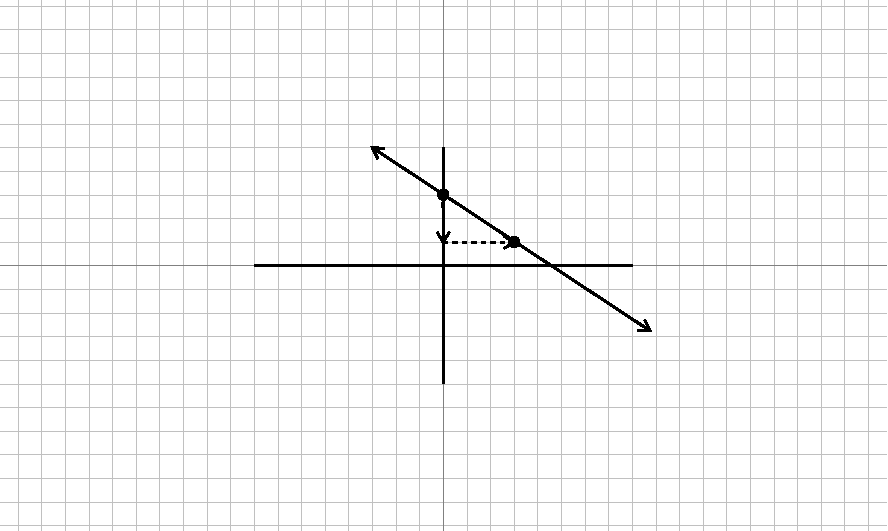
\includegraphics[scale=.9,bb = 115 65 310 190, clip=true]{II_1_4a-1.eps}
    
 Identify the point where the graph crosses the $y$-axis (0,3).\\ This means the $y$-intercept is 3.\pp
    
 Identify one other point and draw a slope triangle to find the slope.\pp
The slope is $m=- \frac{2}{3}$.
  \end{multicols}

\begin{center}
  $y = m x + b\qquad\qquad\qquad$ Slope-intercept equation\\
  $y = - \frac{2}{3} x + 3\qquad\qquad\qquad$ Our solution\qquad\qquad~~~
\end{center}

 % y = - \frac{2}{3} x + 3 &  & \tmop{Our} \tmop{solution}
%\end{eqnarray*}
%\end{example}

 We can also move the opposite direction, using the equation identify the slope
and $y$-intercept and graph the equation from this information. However, it will
be important for the equation to first be in slope intercept form. If it is
not, we will have to solve it for $y$ so we can identify the slope and the
$y$-intercept.

\begin{example}\label{Lin58}~~~Write the equation $2x=4y=6$ in slope-intercept form.
  
  \begin{eqnarray*}
    2 x - 4 y = 6~~ &  & \tmop{Solve} \tmop{for} y\\
    \tmmathbf{\underline{- 2 x ~~~~- 2 x}} &  & \tmop{Subtract} 2 x \tmop{from} \tmop{both}
    \tmop{sides}\\
    - 4 y = - 2 x + 6 &  & \tmop{Put} x \tmop{term} \tmop{first}\\
    \tmmathbf{\overline{- 4} ~~~~ \overline{- 4} ~~ \overline{- 4}} &  & \tmop{Divide~}
    \tmop{each} \tmop{term} \tmop{by} - 4\\
    y = \frac{1}{2} x - \frac{3}{2} &  & \tmop{Our} \tmop{solution}
  \end{eqnarray*}
\end{example}

 Once we have an equation in slope-intercept form we can graph it by first
plotting the $y$-intercept, then using the slope, finding a second point and
connecting the dots.

\begin{example}\label{Lin59}~~~Graph $y=\displaystyle\frac{1}{2}x-4$.
  \begin{eqnarray*}
    y = m x + b&  & \tmop{Slope} - \tmop{intercept} \tmop{equation}\\
    m = \frac{1}{2},~ b = - 4 &  & \tmop{Identify} \tmop{the} \tmop{slope},~ m, \tmop{and} \tmop{the} y - \tmop{intercept},~ b
  \end{eqnarray*}
  \begin{center}
	Now make the graph.
	\end{center}
	\begin{multicols}{2}~\par
    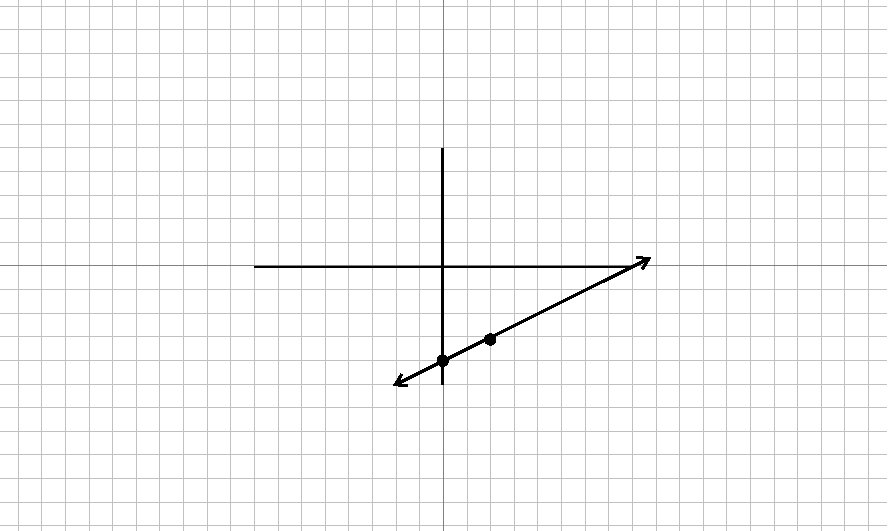
\includegraphics[scale=.9,bb = 115 65 310 190, clip=true]{II_1_4a-2.eps}
    
     Starting with a point at the \\
		$y$-intercept of $- 4$.\\
    
     Then use the slope $\frac{\tmop{rise}}{\tmop{run}}$, so we will rise 1
    unit and run 2 units to find the next point.\\
    
     Once we have both points, connect the dots to get our graph.
  \end{multicols}
\end{example}

\pp

 {\tmstrong{World View Note:}} Before our current system of graphing, French
Mathematician Nicole Oresme, in 1323 suggested graphing lines that would look
more like a bar graph with a constant slope!\pp

\begin{example}\label{Lin60}~~~Graph $3x+4y=12$.
  \begin{eqnarray*}
    3 x + 4 y = 12~~ &  & \tmop{Not} \tmop{in} \tmop{slope-intercept} \tmop{form}\\
    \tmmathbf{\underline{- 3 x ~~~~~~- 3 x}} &  & \tmop{Subtract} 3 x \tmop{from} \tmop{both}
    \tmop{sides}\\
    4 y = - 3 x + 12 &  & \tmop{Put} \tmop{the} x \tmop{term} \tmop{first}\\
    \tmmathbf{\overline{4} ~~~~~~~ \overline{4} ~~~~~ \overline{4}}~ &  & \tmop{Divide} \tmop{each}
    \tmop{term} \tmop{by} 4\\
    y = - \frac{3}{4} x + 3 &  & \tmop{Now~in} \tmop{slope} - \tmop{intercept}
    \tmop{form}\\
    m = - \frac{3}{4},~ b = 3 &  & \tmop{Identify} m \tmop{and} b
  \end{eqnarray*}
  \begin{center}
Now make the graph.
	\end{center}
\end{example}
  \begin{multicols}{2}
	~\par
    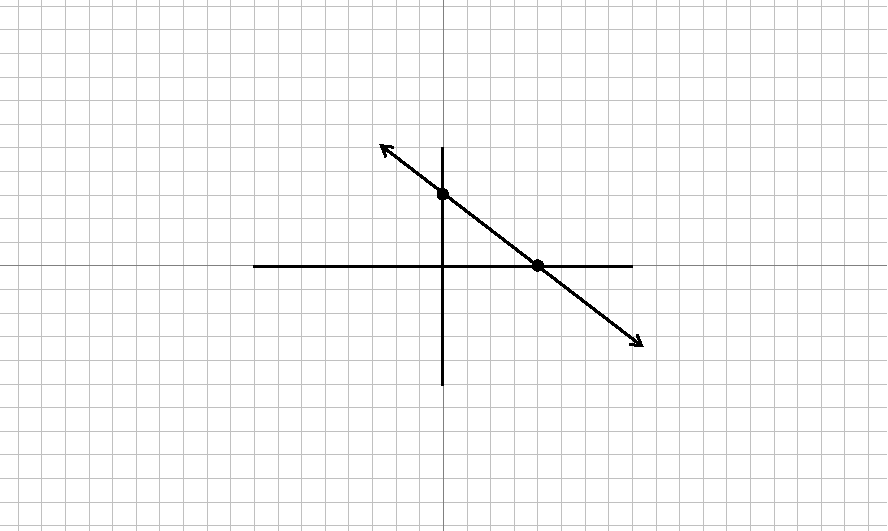
\includegraphics[scale=.9,bb = 115 65 310 190, clip=true]{II_1_4a-3.eps}
    
    \
    
     Starting with a point at the \\$y$-intercept of $3$.\\
    
 Then use the slope $\frac{\tmop{rise}}{\tmop{run}}$, but its negative so
    it will go downhill, so we will drop 3 units and run 4 units to find the
    next point.\\
    
     Once we have both points, connect the dots to get our graph.
  \end{multicols}

 We want to be very careful not to confuse using slope to find the next point
with use a coordinate such as $(4, - 2)$ to find an individual point.
Coordinates such as $(4, - 2)$ start from the origin and move horizontally
first, and vertically second. Slope starts from a point on the line that could
be anywhere on the graph. The numerator is the vertical change and the
denominator is the horizontal change.\pp

 Lines with zero slope or no slope can make a problem seem very different.  Such lines are horizontal.
A horizontal line will have a slope of zero which when
multiplied by $x$ gives zero. So the equation simply becomes $y = b$ or $y$ is
equal to the $y$-coordinate of the graph. If we have no slope, or a vertical
line, the equation can't be written in slope intercept at all because the
slope is undefined. There is no $y$ in these equations. We will simply make
$x$ equal to the $x$-coordinate of the graph.

\begin{example}\label{Lin61}
~\end{example}
  
  \begin{multicols}{2}
    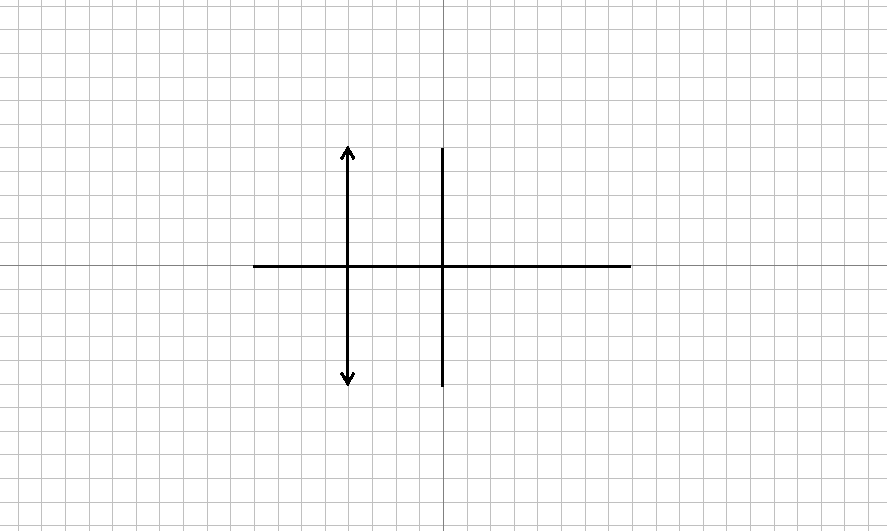
\includegraphics[scale=.9,bb = 115 65 310 190, clip=true]{II_1_4a-4.eps}
    
Give the equation of the line in the graph.\pp 
Because we have a vertical line and no slope there is no slope-intercept equation we can use.\pp
Rather we make $x$ equal to the $x$-coordinate of $- 4$
  \end{multicols}
	\begin{center}
	    Our solution is $x = - 4$.
	\end{center}
%\end{example}
